\phantomsection
\subsection*{SVM formula deduction}
\addcontentsline{toc}{subsection}{SVM formula deduction}
\label{sec:svm_formula}

We have a cloud of points in a higher-dimensional space and we want a plane that separates the ones marked human and the ones marked as murine\futnotetext\footnotetext{Those are what we call tags: $+1$ for human and $-1$ for murine chains.}. But we do not only want \emph{one} that does that, we need the plane that does that the best: that is the one that maximizes the distance to the closest points.

We \emph{must} assume that the two groups of points are separable by a plane in our space and let us say the distance\futnotetext\footnotetext{Distance from one set to another is defined as the minimum distance from one point of one set to a point of the other one. Those two (or more) points will be called support vectors.} between the two clouds is $2d$; we will need this later.

Our solution will have the form:
\begin{equation*}
    \bm w^T \bm X + b = 0,
\end{equation*}
where $\bm w$ is the vector perpendicular to the solution plane, $\bm X$ is a variable-coordinate vector and $b$ is a real number we will call bias.

Since the norm of $\bm w$ is arbitrary, we can set $\left\| \bm w \right\|=  1/d$. Thus, any of our data points inputted in the function $\bm{x}\mapsto \left|   \bm w^T \bm{x}+b\right|  $ will give an output greater or equal to $1$ (the nearest ones will give 1, otherwise strictly greater than 1).\futnotetext\footnotetext{Notice that $\bm x$ and $\textbf x$ are different, in fact, $\bm x_i$ is the data point $\textbf{x}_i $ in the transformed space ($\varphi(\textbf{x}_i)=\bm x_i$, being $\varphi$ the transformation of our space such that $\varphi(\textbf{x}_i)\cdot\varphi(\textbf{x}_j)=\bm x_i^T\bm x_j=\operatorname k(\textbf x_i,\textbf x_j)$).}

Furthermore, we know whether the result will be negative and then inverted by the absolute value. The ones such that \(\bm w^T \bm{x}_i+b\le -1\) will have also the negative tag: $s_i=-1$. Thus, $$\left(   \bm w^T \bm{x}_i+b\right)s_i \ge 1\ \forall i\in\{1,\dots,n\}.$$

Maximizing $d$ is equivalent to minimizing $\left\| \bm w \right\|$, which is again equivalent to minimizing \(\frac{1}{2}\left\| \bm w \right\| ^2\), this will come handy after some computations.

We have an optimization problem subject to restrictions:
\begin{equation*}
    \underset{\bm w,\ b}{\text{minimize}} \ \frac{1}{2}\left\| \bm w \right\| ^2,\qquad
    \text{subject to} \left( \bm w^T \bm{x}_i + b \right) s_i\ge 1 \ \forall i \in\{1,\dots,n\}
\end{equation*}

We define the Lagrangian with the classification margin:
\begin{equation*}
\mathcal{L}(\bm{w}, b, \lambda) = \frac{1}{2} \|\bm{w}\|^2 - \sum_{i=1}^n \lambda_i (s_i(\bm{w}^T \bm{x}_i + b) - 1)
\end{equation*}

We set the partial derivatives to 0:
\begin{equation*}
\nabla_{\bm{w}} \mathcal{L} = 0 \implies \bm{w} = \sum_{i=1}^n \lambda_i s_i \bm{x}_i
\qquad\qquad
\frac{\partial \mathcal{L}}{\partial b} = 0 \implies \sum_{i=1}^n \lambda_i s_i = 0
\end{equation*}

We substitute $\bm{w}$ back into the Lagrangian and apply the restriction for $b$:
\begin{equation*}
\mathcal{L}(\lambda_1,\dots,\lambda_n) = \frac{1}{2} \sum_{i=1}^n \sum_{j=1}^n \lambda_i \lambda_j s_i s_j \bm{x}_i^T \bm{x}_j - \sum_{i=1}^n \sum_{j=1}^n \lambda_i \lambda_j s_i s_j \bm{x}_i^T \bm{x}_j - b \sum_{i=1}^n \lambda_i s_i + \sum_{i=1}^n \lambda_i
\end{equation*}

We simplify  to obtain the dual formulation:
\begin{equation*}
\mathcal{L}(\lambda_1,\dots,\lambda_n) = \sum_{i=1}^n \lambda_i - \frac{1}{2} \sum_{i=1}^n \sum_{j=1}^n \lambda_i \lambda_j s_i s_j \bm{x}_i^T \bm{x}_j,
\end{equation*}

We use our kernel notation for the inner products:
\begin{equation*}
\mathcal{L}(\lambda_1,\dots,\lambda_n) = \sum_{i=1}^n \lambda_i - \frac{1}{2} \sum_{i=1}^n \sum_{j=1}^n \lambda_i \lambda_j s_i s_j \operatorname{k}(\textbf{x}_i, \textbf{x}_j),
\end{equation*}
\begin{equation*}
    \text{with } \sum_{i=1}^n \lambda_i s_i = 0 \text{ and } \lambda_i\ge0\ \forall i\in \left\{ 1,\dots,n \right\} 
\end{equation*}

This way we find the lagrange multipliers, maximizing the Lagrangian subject to the restrictions given.

Usually, this optimization problem is solved via quadratic programming, which takes advantage of some of the properties of the kernel (like smoothness and uniform concavity, $f''(x)<0$, with respect to the inner product). However, it will be convenient not to have these constraints for some other kernels we will be crafting. Instead of the common quadratic programming for maximization, we will be using a simulated annealing algorithm (for minimization of the negated function).

\phantomsection
\subsection*{SVM simulated annealing}
\addcontentsline{toc}{subsection}{SVM simulated annealing}
\label{sec:svm_annealing}

The hard part is out of the way: we have our function to optimize
\begin{equation*}
    E(\lambda) = \frac{1}{2}\sum_{k=1}^{n}\sum_{m=1}^{n} \lambda _k \lambda _m s_ks_m[G]_{k,m} - \sum_{k=1}^{n} \lambda _k 
\end{equation*}


Now we just need the stochastic change function.

Let's consider the naïve approach. We could write a loop that adds a random increment to every $\lambda_i$ except the last one, and then forces the constraint to hold by setting that final one to:
$$
\lambda_n = -s_n \sum_{i=1}^{n-1} \lambda_i s_i
$$
Watch out: for this step to actually be valid, the result must fall between $0$ and our upper limit hyperparameter $\lambda_t$ (the one from the SVM results section). Randomly hitting a valid number this way is incredibly slow and mathematically unlikely.

Instead, we made the algorithm about 20\futnotetext\footnotetext{This was measured comparing computation times of the full simulated annealing, going from 40 minutes all the way down to 2 minutes, and also having applied the following optimization on the energy function.} times faster by picking just two random indices, $i$ and $j$. We apply a random increment to $\lambda_i$ and simply adjust $\lambda_j$ to balance it out and satisfy the constraint. 

Say in the next iteration \(\lambda _i\mapsto \lambda _i'\) and \(\lambda _j\mapsto \lambda _j'\) and define the difference \(\Delta \lambda_i=\lambda _i'- \lambda _i=d\). We must satisfy \(\sum_{}^{} \lambda _ks_k=0\), therefore \(\lambda _is_i+\lambda _js_j=\lambda _i's_i+\lambda _j's_j\), and so:
\begin{equation*}
    \Delta \lambda_j = \lambda _j'-\lambda _j=-ds_is_j
\end{equation*}


We take advantage of this localized change in our energy function as well. Calculating the product $\mathbf{x}^TG \mathbf{x}$ from scratch to get $E$ at every single step is computationally expensive and bogs everything down. Since we are only modifying two components of the $\lambda$ vector, we need not redo all our math.

Thus, we have the energy before the change \(E(\lambda )\), just like already shown, and the energy after a change \(\Delta \lambda\) is
\begin{equation*}
    E(\lambda+\Delta \lambda) =
    \frac{1}{2}\sum_{k\neq i,j}^{n} \sum_{m\neq i,j}^{n} \lambda _k \lambda _m s_ks_m[G]_{k,m} -\sum_{k\neq i,j}^{n} \lambda _k + E_1' + E_2' + E_3'
\end{equation*}

The  not explicitly shown quantities, \(E_i\), are the ones that were modified (with the change in the \(i\)-th and \(j\)-th components) with the addition of the \(\Delta \lambda\) to the imput. Starting with the easy one, from the \(\lambda_k\) summation:
\begin{equation*}
    E_1' = -\lambda _i'-\lambda _j'
\end{equation*}

Now with the double summation, we want the addends that contain a \(\lambda _i\) or (inclusive) \(\lambda_j\). We'll do it first with the terms that only contain one modified lambda.
\begin{align*}
    E_2' &= \frac{1}{2}\sum_{m\neq i,j}^{n} \left(  \lambda _i'\lambda _ms_is_m[G]_{i,m} +  \lambda _j'\lambda _ms_js_m[G]_{j,m}  \right)+
    \frac{1}{2}\sum_{k\neq i,j}^{n}  \left( 
    \lambda _k \lambda _i's_ks_i[G]_{k,i} +
    \lambda _k \lambda _j's_ks_j[G]_{k,j}
     \right) \\
     &= \sum_{\beta\neq i,j}^{n} \left(  \lambda _i'\lambda _\beta s_is_\beta [G]_{i,\beta } +  \lambda _j'\lambda _\beta s_js_\beta [G]_{j,\beta }  \right)
\end{align*}
Using \(F_\alpha = \sum_{\beta\neq i,j}^{n}\lambda _\beta s_\beta [G]_{\beta ,\alpha } \)\futnotetext\footnotetext{In the code, we use \(F_\alpha = \sum_{\beta=1}^{n}\lambda _\beta s_\beta [G]_{\beta ,\alpha } \) which can be proven to be equivalent in the final expression.}:
\begin{equation*}
    E_2 = \lambda _i's_i F_i + \lambda _j's_jF_j
\end{equation*}


Finally, the terms that contain both lambdas modified:
\begin{equation*}
    E_3'=\frac{1}{2}\lambda _i'^2s_i^2[G]_{i,i}+
    \frac{1}{2}\lambda _j'^2s_j^2[G]_{j,j}+
    2\cdot \frac{1}{2}\lambda_i'\lambda_j's_is_j[G]_{i,j}=
    \frac{1}{2}\lambda _i'^2[G]_{i,i}+
    \frac{1}{2}\lambda _j'^2[G]_{j,j}+
    \lambda_i'\lambda_j's_is_j[G]_{i,j}
\end{equation*}

We take the difference \(\Delta E (\lambda)=E(\lambda+\Delta \lambda)-E(\lambda)\):
\begin{align*}
    \Delta E(\lambda )
    &= E_1'+E_2'+E_3'-\left( E_1+E_2+E_3 \right) 
    =\Delta E_1 + \Delta E_2 +\Delta E_3
    \\
    \Delta E_1&= -\lambda _i'-\lambda _j' - (-\lambda _i-\lambda _j)=-d(1-s_is_j)\\
    \Delta E_2&= \lambda _i's_i F_i + \lambda _j's_jF_j - (\lambda _i's_i F_i + \lambda _j's_jF_j) = d s_i (F_i - F_j)\\
    \Delta E_3&= 
    \frac{1}{2}(\lambda _i'^2-\lambda _i^2)[G]_{i,i}+
    \frac{1}{2}(\lambda _j'^2-\lambda _j^2)[G]_{j,j}+
    (\lambda_i'\lambda_j'-\lambda _i \lambda _j)s_is_j[G]_{i,j}=\\
    &=\frac{1}{2} d^2 ([G]_{i,i} + [G]_{j,j} - 2 [G]_{i,j})
\end{align*}

Thus:
\begin{equation*}
    \Delta E(\lambda)=
    ds_i(F_i-F_j)-d(1-s_is_j)+\frac{1}{2} d^2 \left([G]_{i,i} + [G]_{j,j} - 2 [G]_{i,j}\right)
\end{equation*}






% We can keep the last computed energy and just add or subtract the change:
% $$
% \Delta E = -d (1 - s_is_j) + d s_i (F_i - F_j) + \frac{1}{2} d^2 ([G]_{i,i} + [G]_{j,j} - 2[G]_{i,j})
% $$
% Here, $d$ is our proposed increment $\Delta \lambda_i$, the class labels are $s \in \{-1, 1\}$, $G$ is the kernel Gram matrix, and $F_k = \sum_m \lambda_m s_m [G]_{k,m}$ acts as our running partial evaluation for the $k$-th sample.

% Let's break down exactly where this comes from. Because of the linear constraint $\sum_{k} \lambda_k s_k = 0$, shifting $\lambda_i$ by $d$ immediately forces $\Delta \lambda_j$ to be $-d s_i s_j$. We can expand the exact difference 
% $$
% \Delta E = E(\lambda + \Delta\lambda) - E(\lambda)
% $$
% from our dual objective energy 
% $$
% E(\lambda) = \frac{1}{2} \sum_{k,m} \lambda_k \lambda_m s_k s_m [G]_{k,m} - \sum_{k} \lambda_k
% $$
% directly into the components of our shortcut equation. First, let's look at the linear portion $-\sum \lambda_k$. The variation here is simply:
% $$
% -(\Delta \lambda_i + \Delta \lambda_j) = -(d - d s_i s_j) = -d (1 - s_i s_j)
% $$
% Next, consider the cross interaction between the new increments and the existing values of all the other multipliers in the quadratic form. This gives $\Delta \lambda_i s_i F_i + \Delta \lambda_j s_j F_j$. Since $s_j^2 = 1$, it simplifies neatly to $d s_i (F_i - F_j)$. Finally, the increments also interact with themselves. If we expand the quadratic form exclusively for our modified components $i$ and $j$, we get:
% $$
% \frac{1}{2} \left[ (\Delta \lambda_i s_i)^2 [G]_{i,i} + (\Delta \lambda_j s_j)^2 [G]_{j,j} + 2 (\Delta \lambda_i s_i)(\Delta \lambda_j s_j) [G]_{i,j} \right]
% $$
% which collapses straight into $\frac{1}{2} d^2 ([G]_{i,i} + [G]_{j,j} - 2 [G]_{i,j})$.

By tracking these $F$ values, which only require an $\mathcal{O}(n)$ update whenever we accept a move, we bring the complexity of calculating the energy difference for any proposed stochastic jump crashing down from $\mathcal{O}(n^2)$ to just $\mathcal{O}(1)$. This mathematical shortcut is precisely what makes simulating millions of iterations computationally viable.










\phantomsection
\subsection*{SVM decision function}
\addcontentsline{toc}{subsection}{SVM decision function}
\label{sec:svm_decision}

For our decision function we just want to know which side of the plane is on. We achieve that plugging the new data point into our plane equation:
\begin{equation*}
    \bm w^T \bm{x} +b = \left( \sum_{i=1}^n \lambda_i s_i \bm{x}_i^T \right) \bm{x}+b
    =
    \sum_{i=1}^n \lambda_i s_i \bm{x}_i^T \bm{x}+b
    =
    \sum_{i=1}^n \lambda_i s_i \operatorname{k}(\textbf x_i, \textbf x)+b
\end{equation*}


\begin{equation*}
    f:\textbf  x\mapsto b + \sum_{i=1}^n\lambda_i s_i \operatorname k(\textbf x_i,\textbf x)
\end{equation*}

Also, since $(\bm w^T \bm x_p + b)s_p = 1$ for some support vector $\textbf{x} _p$, 
expanding $\bm w$:
\begin{equation*}
    b=s_p-\sum_{i=1}^n \lambda_i s_i \operatorname k(\textbf x_i, \textbf x_p)
\end{equation*}














\phantomsection
\subsection*{SVM kernel function comparison}
\addcontentsline{toc}{subsection}{SVM kernel function comparison}
\label{sec:svm_comparison}

\begin{figure}[H]
    \centering
    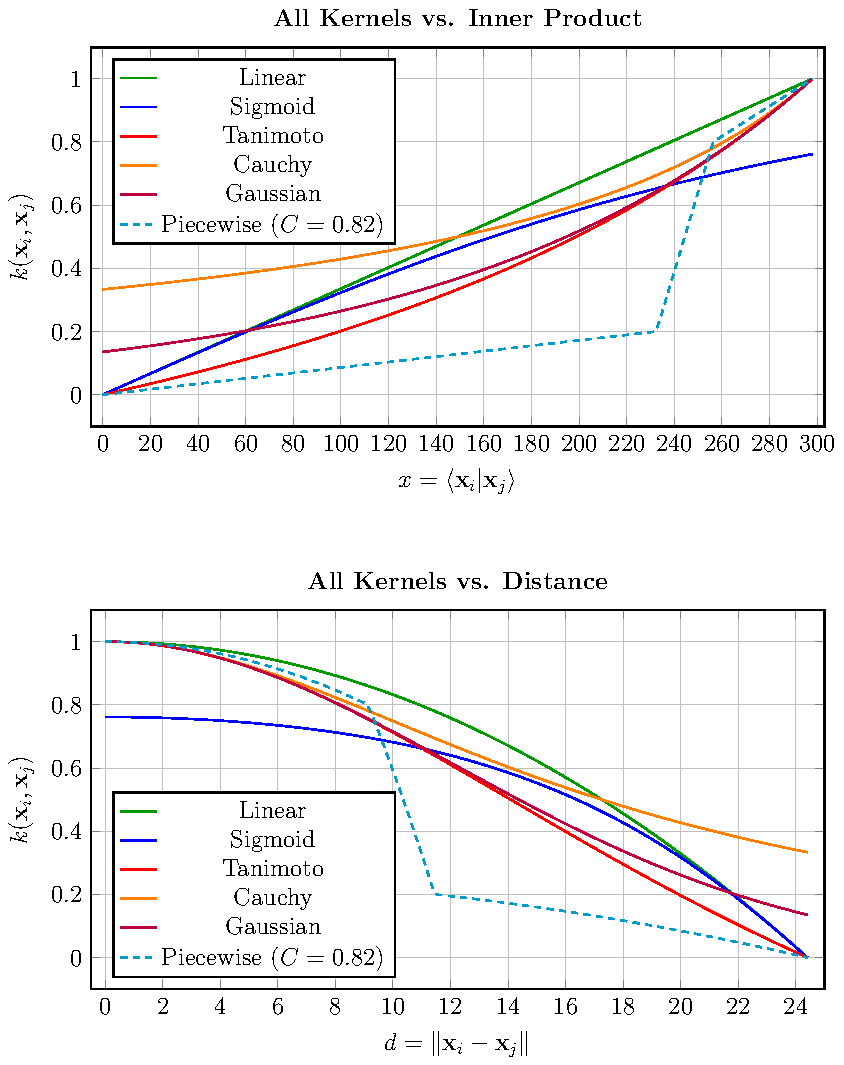
\includegraphics[width=.9\textwidth]{images/kernel_functions.pdf}
\end{figure}

\phantomsection
\subsection*{Piecewise kernels performance}
\addcontentsline{toc}{subsection}{Piecewise kernels performance}
\label{sec:piecewise_results_table}

\begin{table}[H]
    \centering
    \renewcommand{\arraystretch}{1.4}
    \begin{tabular}{lcccc} \cline{2-5}
        Kernel parameters & Accuracy & $\text{F1}_\text{H}$ & $\text{F1}_\text{M}$ & $\mathcal Q$ \\ \hline \hline
        Piecewise ($C=0.80$, $W=0.20$) & $0.9880$ & $0.9903$ & $0.9844$ & $0.9372$ \\ \hline
        Piecewise ($C=0.80$, $W=0.08$) & $0.9850$ & $0.9878$ & $0.9806$ & $0.9357$ \\ \hline
        Piecewise ($C=0.82$, $W=0.08$) & $0.9895$ & $0.9915$ & $0.9865$ & $0.9288$ \\ \hline
        Piecewise ($C=0.84$, $W=0.08$) & $0.9895$ & $0.9915$ & $0.9865$ & $0.9228$ \\ \hline
        Piecewise ($C=0.78$, $W=0.08$) & $0.9820$ & $0.9853$ & $0.9769$ & $0.9395$ \\ \hline
    \end{tabular}
    \caption{Performance of the custom piecewise kernels on the test dataset (668 samples), including the quadratic certainty score $\mathcal Q$.}
    \label{tab:piecewise_results}
\end{table}

\phantomsection
\subsection*{Permutation importance}
\addcontentsline{toc}{subsection}{Permutation importance}
\label{sec:permutation_importance_table}

\begin{table}[H]
    \centering
    \renewcommand{\arraystretch}{1.4}
    \begin{tabular}{lccc} \cline{2-4}
        Kernel & Accuracy drop & $\text{F1}_\text{H}$ drop & $\text{F1}_\text{M}$ drop \\ \hline \hline
        Tanimoto & $+0.0087$ & $+0.0072$ & $+0.0109$ \\ \hline
        Gaussian (RBF) & $+0.0085$ & $+0.0070$ & $+0.0106$ \\ \hline
        Linear & $+0.0060$ & $+0.0050$ & $+0.0075$ \\ \hline
        Cauchy & $+0.0055$ & $+0.0046$ & $+0.0069$ \\ \hline
        Piecewise ($C=0.80$, $W=0.20$) & $+0.0051$ & $+0.0042$ & $+0.0064$ \\ \hline
        Sigmoid & $+0.0049$ & $+0.0041$ & $+0.0061$ \\ \hline
        Piecewise ($C=0.78$, $W=0.08$) & $+0.0031$ & $+0.0026$ & $+0.0039$ \\ \hline
        Piecewise ($C=0.84$, $W=0.08$) & $+0.0029$ & $+0.0024$ & $+0.0037$ \\ \hline
        Piecewise ($C=0.80$, $W=0.08$) & $+0.0029$ & $+0.0024$ & $+0.0036$ \\ \hline
        Piecewise ($C=0.82$, $W=0.08$) & $+0.0029$ & $+0.0024$ & $+0.0036$ \\ \hline
    \end{tabular}
    \caption{Permutation importance measured on the test dataset across 500 random shuffles per feature.}
    \label{tab:permutation_importance_appendix}
\end{table}


